\section{IoT as a Socio-technical System}
\label{sec:IoT_socio-techical}

\begin{svgraybox}
	Through this chapter, we review the literature on
	
	1 IoT as socio-technical system and
	
	2 how IoT can support the design and development of the smart grid.
\end{svgraybox}

Since 1999, when Ashton \cite{ashton2011internet} coined the term \textbf{Internet of Things (IoT)}, while he was introducing RFID technology in the context of supply-chain management, the meaning of the term has evolved. Today, International Telecommunication Union (lTU) defines IoT as the worldwide network of interconnected objects uniquely addressable based on standard communication protocols. Such a definition focuses only on the technical side of IoT. From the technical aspect, the IoT can be divided into three following layers:
\begin{itemize}
	\item comprehensive sensing (perception layer),
	\item reliable transmission (network layer), and
	\item intelligent processing (application layer).
\end{itemize}
Nevertheless, the envisioned IoT represents a socio-technical, instead of an only technical system, as the interconnected objects are intended to interact also with people and society \cite{atzori2014smart,Shin2014}. 
However, the focus among engineers and computer scientists when discussing IoT was mainly on the technical side, as is the case with other socio-technical systems.
Interestingly, even some of the ideas for the \textit{Social IoT (SIoT)} \cite{atzori2012social,guinard2010sharing,atzori2014smart} discuss the convergence of social networks with IoT mainly with the intention to optimize the interactions among the IoT objects. There is often very little attention placed in such studies on the interrelationship of IoT with the human psychological and social aspects \cite{atzori2012social,guinard2010sharing}. 

The discussion on IoT should also cover another term that is often used interchangeably -- \textbf{ubiquitous computing}, coined by Weiser \cite{weiser1991computer}. Ubiquitous computing is defined as ``the physical world that is richly and invisibly interwoven with sensors, actuators, displays, and computational elements, embedded seamlessly in the everyday objects of our lives, and connected through a continuous network'' (ibid.). In other words, while the Internet has led to the interconnection of people at an unprecedented scale, the IoT is expected to interconnect also the objects around us, leading to a smart environment \cite{gubbi2013internet}. %We see that researches talking about IoT mainly describe connected devices, while ubiquitous computing focuses on the smart environment in which computing is pervasive. 
%Hence, the two terms take a different stance and focus on different aspects of what is envisioned to become the \textit{Future Internet}. 
The IoT vision put forward by Weiser \cite{weiser1991computer} led to a fruitful new field within computer science (ubiquitous computing). In particular, the original vision suggested that ubiquitous computing can lead to an environment that is predicting and adapting to the people's needs, while the people were considered passive elements (i.e., technological determinism). However, Rogers \cite{rogers2006moving} offered a constructive critique of this vision. Namely, Rogers argued that we should move from a \textit{computing approach} (technical aspects) to a \textit{human approach} (social aspects) in developing the smart environment. Rogers argues: ``To make this happen, however, requires moving from a mindset that wants to make the environment smart and proactive to one that enables people, themselves, to be smarter and proactive in their everyday and working practices.''

The effects of the critique, such as the one by Rogers, are seen in researches increasingly adopting the design of IoT as a socio-technical artifact \cite{ning2011future,guo2012opportunistic,Shin2014,tomasini2017effect}. One human-centric vision is illustrated by the \textit{Opportunistic IoT} \cite{guo2012opportunistic,guo2013opportunistic}. The authors explain that in addition to object-object interaction, the IoT design should consider human-object, human-environment and human-human interactions. Moreover, it is also recognized that the IoT design needs to consider different aspects of human behaviour, such as mobility \cite{tomasini2017effect}, preferences \cite{kowshalya2016community}, and homophily \cite{atzori2012social}. In the light of such ideas, Ortiz et al.\ \cite{ortiz2014cluster} revisit previously introduced ideas of {SIoT} (that still treat IoT only as technical system) and provide a more complete vision of it -- one that treats the IoT as a socio-technical system.

\begin{comment}
	\sidecaption
	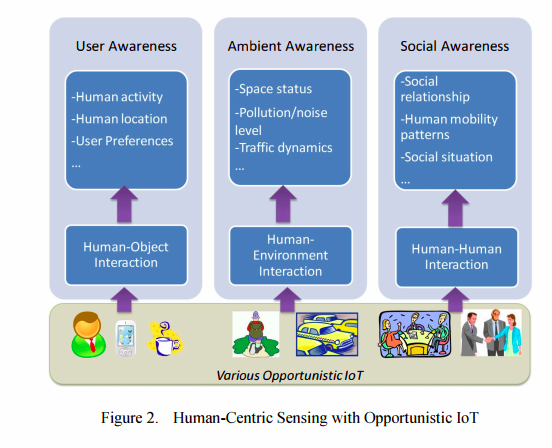
\includegraphics[scale=.55]{img/opprtunisticIoT}
	\caption{Human-centric Opportunistic IoT \cite{guo2012opportunistic}}
	\label{fig:opportunisticIoT} 
\end{comment}

Some of the key ideas in which the visions of IoT as a socio-technical system (SIoT) expand on those visions that treat it only as a technical system are the following. SIoT visions argue that the efforts should be placed on using and integrating the IoT in society and on the user-level, and building new communities of users and technology while considering actual adoption possibilities (versus designing intrusive technology that will not be used in the end). Moreover, the emphasis is on contextual design, so that IoT will be adapted to different psychological, social, legal, policy and other types of factors. Finally, people have to be empowered to embrace the IoT technologies with awareness raising, proper policies and  human-centered design \cite{ning2011future,Shin2014}.


\subsection{IoT for the Smart Grid}
\label{sec:IoTSG}
One of the key application areas of IoT is envisioned for the \textbf{smart grid}. In China, in particular, the largest portion of the IoT market is planned for the development of the smart grid \cite{shin2014socio}. Yun and Yuxin \cite{yun2010research} discuss the possibilities of the IoT to bring about the {smart grid} through sensors, novel telecommunications and computing technologies. The sensors, such as smart, temperature, and illumination meters can collect energy and environmental data. They can also form a high-speed, real-time and bidirectional connection between the consumers, utilities and the electrical grid. Such an improved data collection and communication can support the decision making and in turn improve the overall efficiency of the grid. Interestingly, the technology at the heart of the IoT, the Internet itself, consumes up to 5\% of the total energy spent today in the world. Given the expectation of connecting billions of new devices, this consumption is expected to raise \cite{gubbi2013internet}.	Hence, in addition to its role in optimizing the energy grid, the IoT design itself needs to place accent on sustainability.

%Different innovation layers can be used to describe the smart innovation and development characteristics within the smart cities \cite{zygiaris2013smart}. IoT should play an important role in several of those layers: from the interconnection layer with a number of sensors and actuators, through the integration layer monitoring those smart devices, to the intelligent applications layer making use of the real-time data. 

 IoT can support both the dimensions of demand and supply of energy in the smart grid. Tackling the demand should involve the users \cite{verbong2013smart}. While the focus on technology is still too strong and some smart grid players still perceive the users themselves as the barriers to the smart grid development process, they instead need to understand to what extent the users can act as a solution to the sustainability pathway. IoT is an integral technology in the \textit{smart residential buildings} \cite{schatten2014smart,zygiaris2013smart}. The smart devices that are interconnected and installed in smart buildings, such as smart energy, temperature, and illumination meters are enablers of the smart homes.

IoT is predicted to enable transparent energy consumption information of different services in \textit{smart cities}: from lighting, through public transport, to heating and air conditioning of public spaces \cite{zanella2014internet}. Moreover, the real-time, bidirectional connectivity between the utilities, grid and the users is suggested to lead to the improved overall efficiency of the grid \cite{yun2010research,li2011applications}. Similarly as with IoT in general, we also find visions of smart grid that employ social networks on top of interconnected devices, in this case, the smart meters \cite{ciuciu2012social}. Devices, in general, in the future smart homes and cities are expected to cooperate, actively share their energy and participate in building wide energy management systems \cite{karnouskos2010cooperative}. 

It is apparent how in such a context, where IoT meets the smart grid, innovative services and business applications emerge, but also security, privacy and trust gain novel importance.


